% !Mode:: "TeX:UTF-8"
% !TEX root = tjumain.tex

% \iffalse
% \bibliography{reference/reference.bib} % 欺骗latextools获取bib文件
% \fi

%%%%%%% 正文 %%%%%%%
\chapter{报告摘要}


\chapter{协议实现}

第二周的协议实现主要分为“基本方法实现”、“缓冲区处理”、“日志记录模块”、“读写文件”和两个部分。

\section{方法实现}


\section{接收缓冲区实现}

\section{日志记录模块实现}

\section{读写磁盘文件错误处理}

\section{其他细节实现}






\chapter{实验结果及分析}

\section{手工测试}
我们将 liso\_client 设置为忙等待,及其不会自动关闭 socket 并退出,而是占用着服务器的资源等待着。如图\ref{fig:lab4test1},我们同时开启了 4 个陷入忙等待的客户端对服务器发出请求,服务器仍然能正常处理发出 pipeline 请求的客户端。


\begin{figure}[htbp!]
    \centering 
    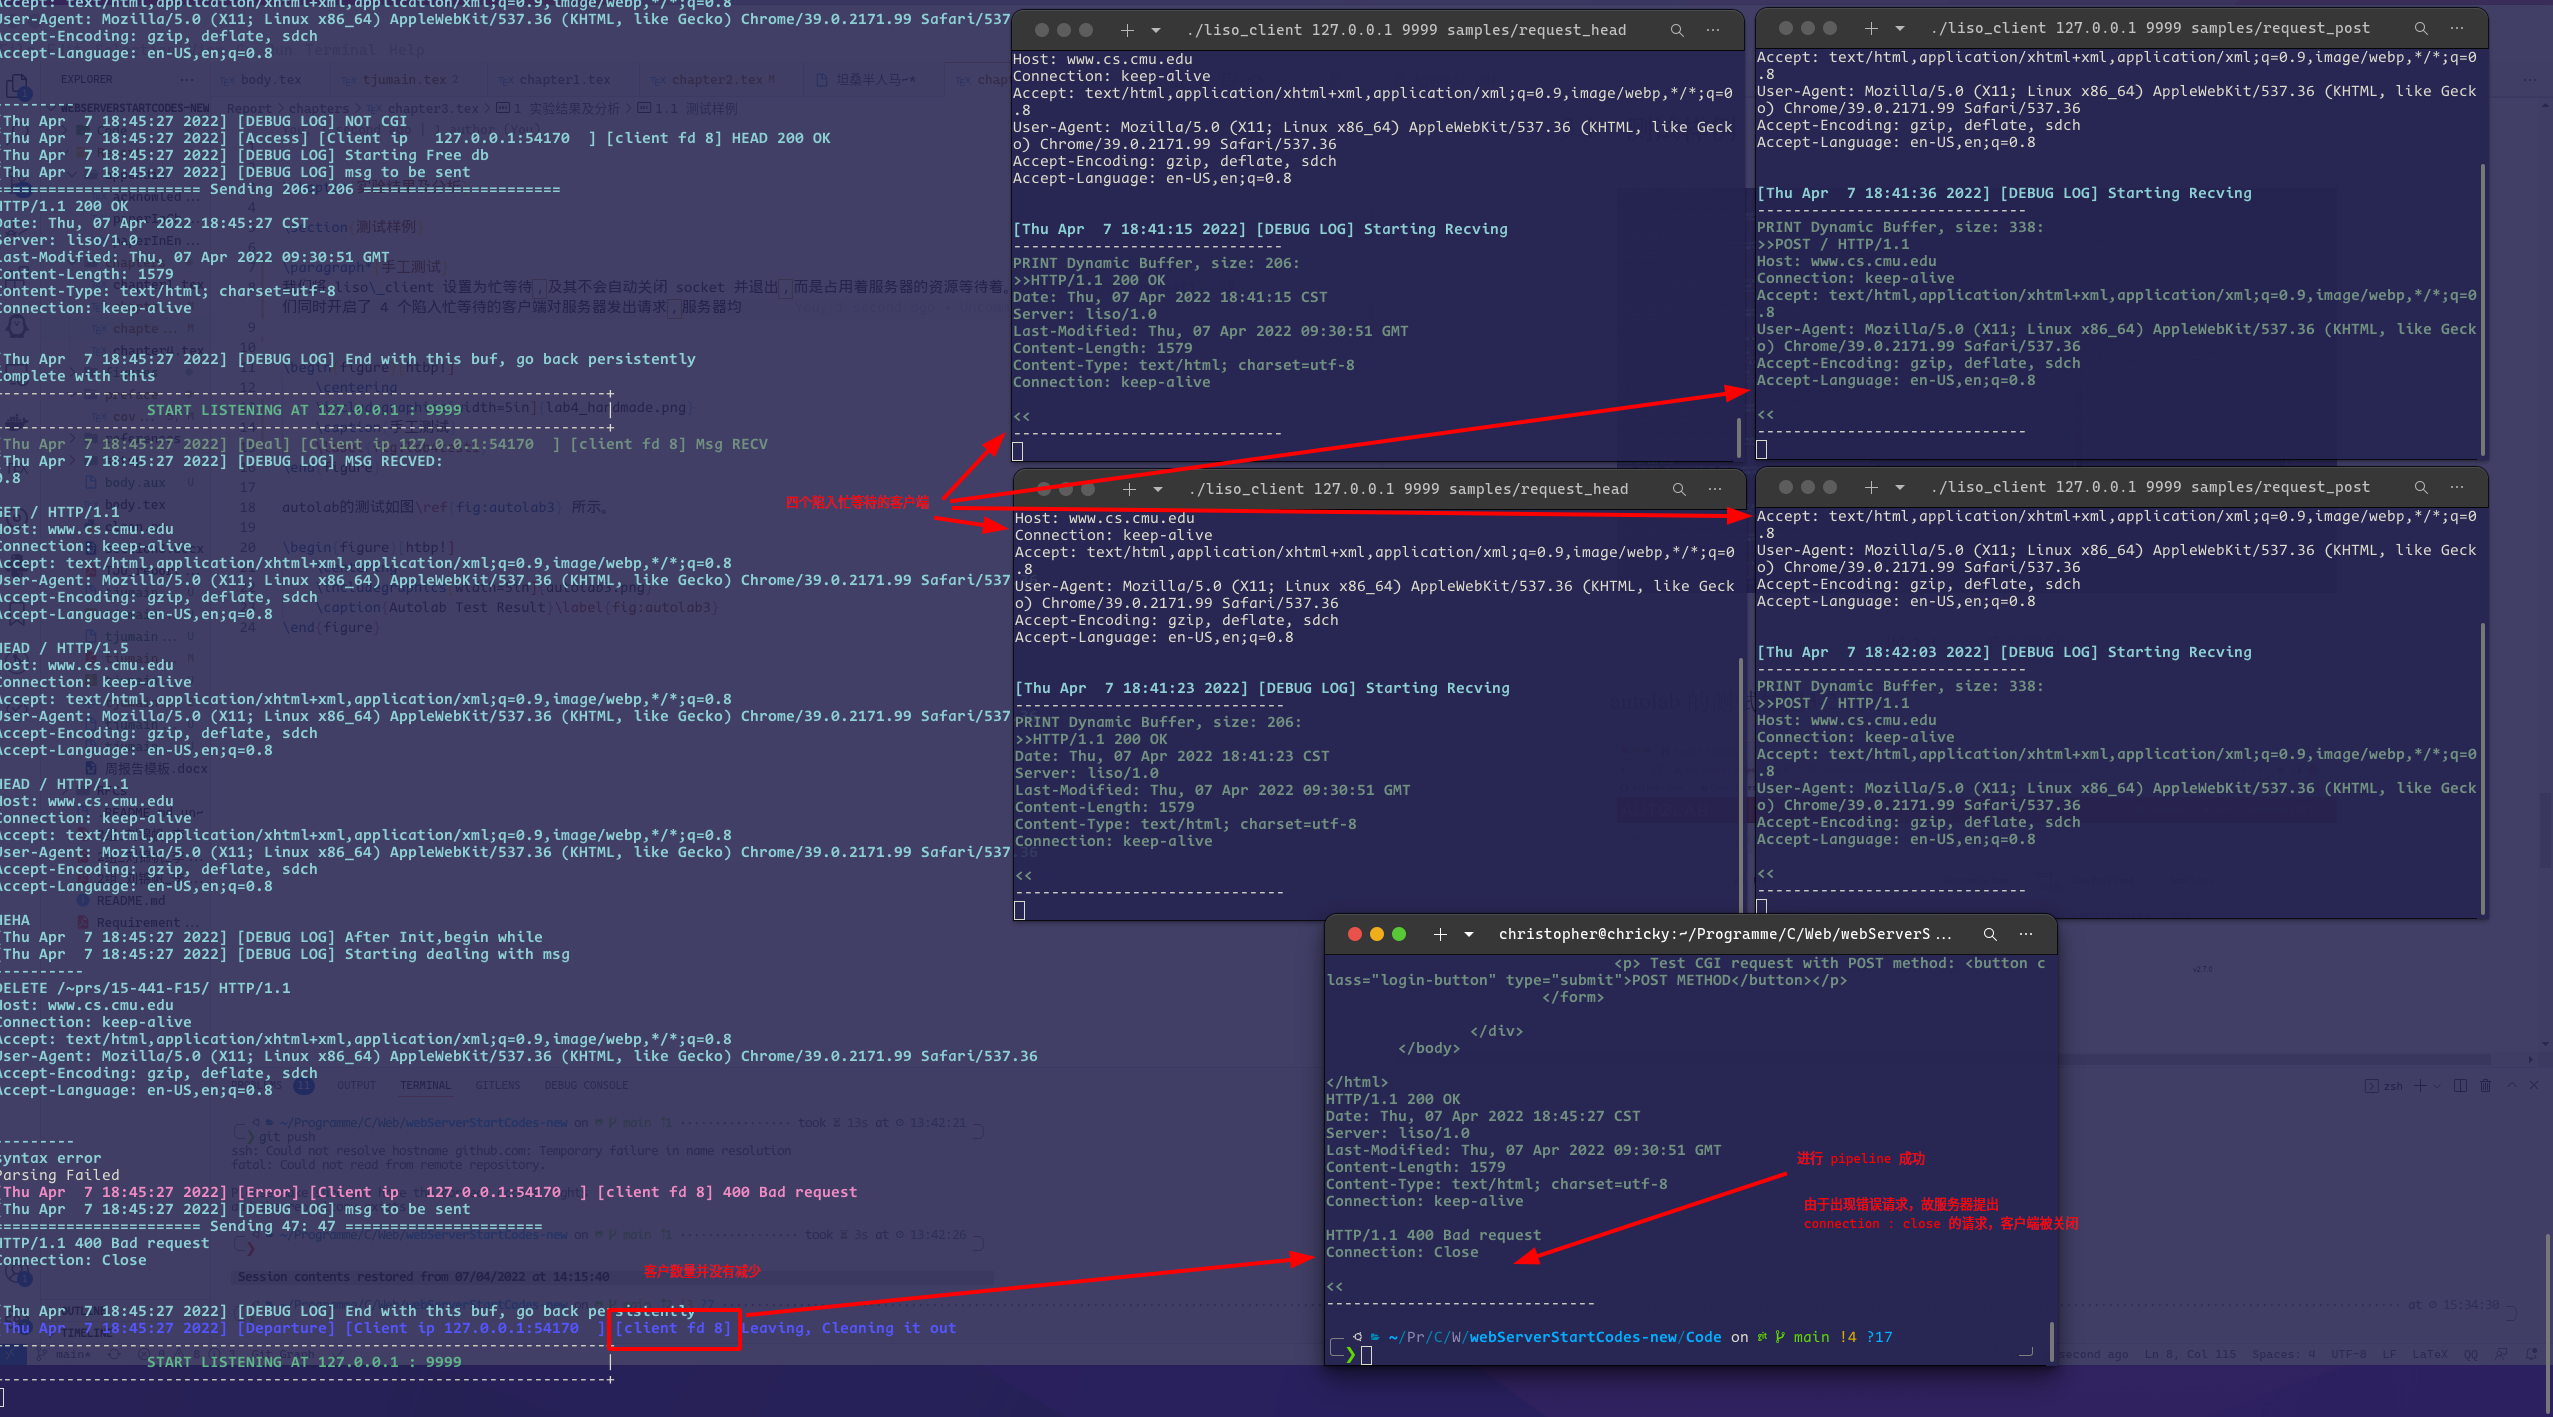
\includegraphics[width=6in]{lab4_handmade.png}
    \caption{手工测试}
    \label{fig:lab4test1}
\end{figure}

\section{Autolab 测试} 如图\ref{fig:autolab4} 所示,在 3月29日 下午完成了初稿,后续修改了部分细节。

\begin{figure}[htbp!]
    \centering
    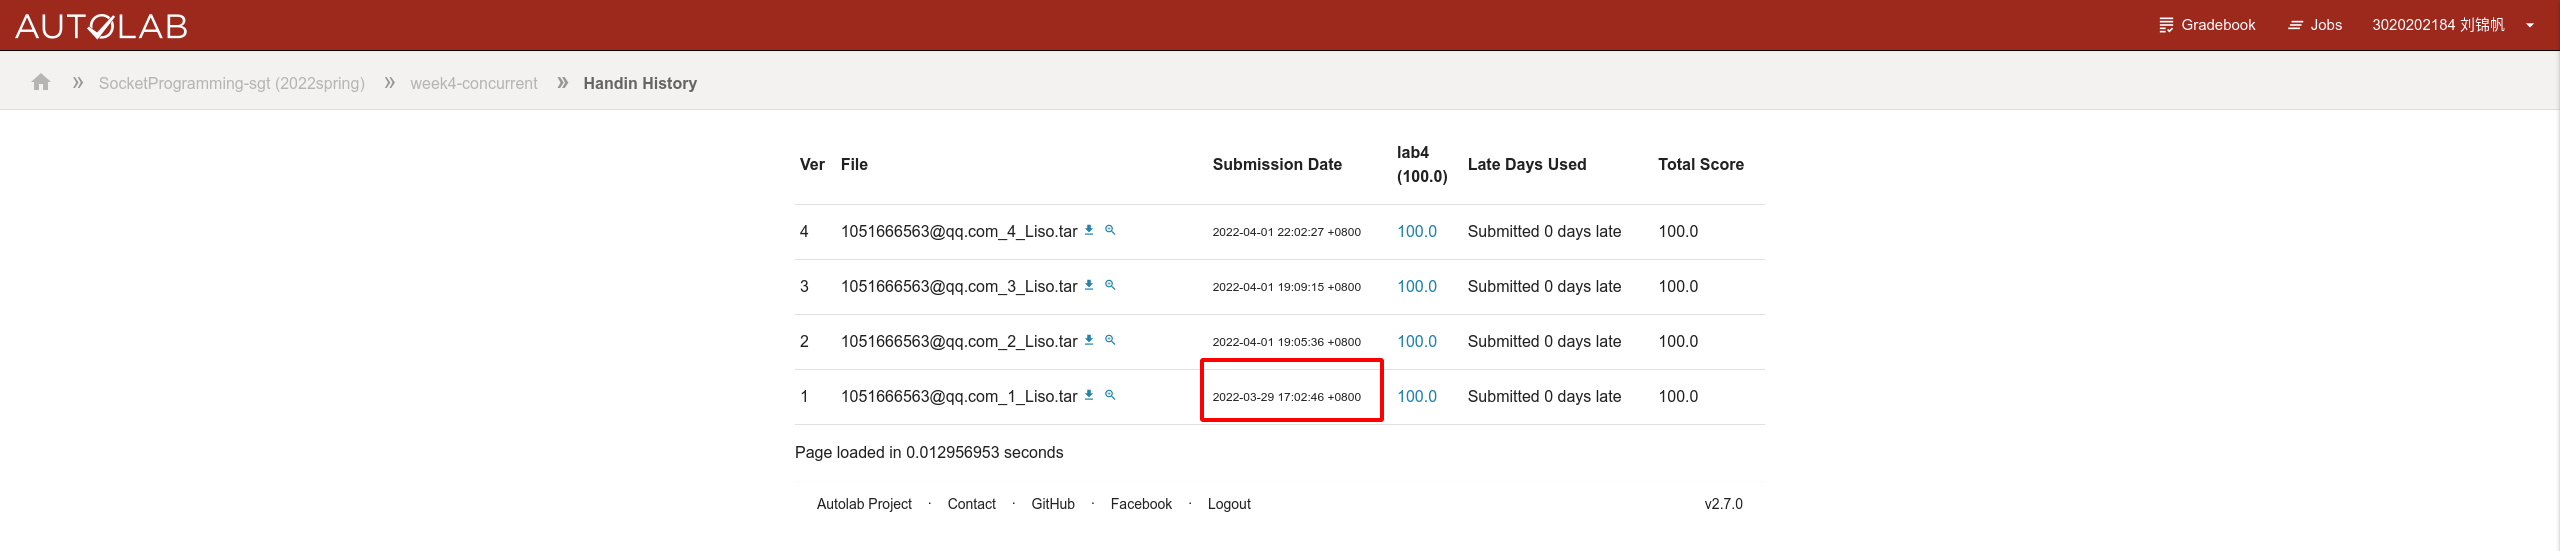
\includegraphics[width=6in]{autolab4.png}
    \caption{Autolab Test Result}\label{fig:autolab4}
\end{figure}

\section{Apache 测试} 

第三周的 liso\_server 由于没有进行并发优化。在测试时由于会一直等待客户端提出退出申请,在测试时会出现 Apache Bench 忙等待。我们分别进行了并发压力测试以及多请求压力测试。测试截图统一放在附录中。

\paragraph*{并发压力测试} 控制总请求数不变的情况下,我们分别进行了并发数量为 10、100 以及 1000 的测试,结果如图所示。如表\ref{tab:parallel} 所示,总请求数量不变情况下,随着并发等级的提高,单个请求的平均反应时间并没有太大的变化。所以可以认为我们的方案是能够解决高并发问题的。

\begin{table}[htbp!]
    \centering
    \begin{tabular}{llll}\hline
      & 并发等级 & 总请求数量 & TPR(ms)   \\\hline
    1 & 10   & 1000  & 0.238 \\
    2 & 100  & 1000  & 0.247 \\
    3 & 1000 & 1000  & 0.222\\
    \hline
    \end{tabular}
    \caption{并发压力测试结果}\label{tab:parallel}
\end{table}

\paragraph*{多请求压力测试} 通过控制并发等级为10不变,改变总请求数量,我们得到了多请求压力测试的结果,如表\ref{tab:multiple}所示。可以轻易看出,在并发等级一定的情况下,总请求数量在100,000量级及以下时,单个请求的平均反应时间都能在正常的范围中。但当请求量达到1,000,000 数量级时,单个请求的平均相应时间则会增加很多,推测是因为请求数量太多,导致频繁接受、删除用户,进而导致反应时间增加。

\begin{table}[htbp!]
    \centering
    \begin{tabular}{llll}\hline
      & 并发等级 & 总请求数量 & TPR(ms)   \\\hline
    1 & 10      & 100       & 0.332 \\
    2 & 10      & 1000      & 0.238 \\
    3 & 10      & 10000     & 0.225\\
    4 & 10      & 100000    & 0.264\\
    5 & 10      & 1000000   & 0.463\\
    \hline
    \end{tabular}
    \caption{多请求压力测试}\label{tab:multiple}
\end{table}

\chapter{协议实现}


\section{第一周——实现简单的 echo web server}

\section{第二周——实现 HEAD、GET、POST 方法}

\section{第三周——实现HTTP的并发请求}

\section{第四周——实现多个客户端的并发处理}



% \chapter{实验展示}


% \begin{figure}[htbp!]
%     \centering
%     \subfigure[Screemshot for Lab2.1]{\includegraphics[width=2.1in]{figures/wireshark1.png}}
%     \subfigure[Screemshot for Lab2.2]{\includegraphics[width=2.1in]{figures/wireshark2.png}}
%     \subfigure[Screemshot for Lab2.3]{\includegraphics[width=2.1in]{figures/wireshark3.png}}
%     \subfigure[Screemshot for Lab2.4]{\includegraphics[width=2.1in]{figures/wireshark4.png}}
%     \subfigure[Screemshot for Lab2.5]{\includegraphics[width=2.1in]{figures/wireshark5.png}}

%     \caption{Wireshak Application Screemshots}\label{fig:Wireshak Application Screemshots}
%     \vspace{-1em}
% \end{figure}

% \chapter{Q\&A}

% \section{The Basic HTTP GET/response interaction}



% \begin{enumerate}
%     \item Is your browser running HTTP version 1.0 or 1.1? What version of HTTP is the  server running?
    
%     \textbf{Answer:} Both are running HTTP version 1.1 
    
%     \item What languages (if any) does your browser indicate that it can accept to the server?
    
%     \textbf{Answer:} 简体中文(繁体),英文(US)。
    
%     \item What is the IP address of your computer? Of the gaia.cs.umass.edu server?

%     \textbf{Answer:}\\
%     My Computer: $172.23.170.212$\\
%     Server: $128.119.245.12$

%     \item What is the status code returned from the server to your browser?
    
%     \textbf{Answer:} Status Code: 200

%     \item What is the status code returned from the server to your browser?
    
%     \textbf{Answer:} Last-Modified: Sun, 13 Mar 2022 06:59:02 GMT

%     \item How many bytes of content are being returned to your browser?
    
%     \textbf{Answer:} 128 bytes

%     \item By inspecting the raw data in the packet content window, do you see any headers within the data that are not displayed in the packet-listing window? If so, name one.
    
%     \textbf{Answer:} No

% \end{enumerate}


% \section{The HTTP CONDITIONAL GET/response interaction}

% \begin{enumerate}
%     \item[8] Inspect the contents of the first HTTP GET request from your browser to the 
%     server. Do you see an “IF-MODIFIED-SINCE” line in the HTTP GET?

%     \textbf{Answer:} We see no "IF-MODIFIED-SINCE" line in the HTTP GET.

%     \item[9] Inspect the contents of the server response. Did the server explicitly return the 
%     contents of the file? How can you tell?

%     \textbf{Answer:} Yes, it did. We may see the whole HTML file in the content field. (Which shall be shown in the appendix section)

%     \item[10]  Now inspect the contents of the second HTTP GET request from your browser to 
%     the server. Do you see an “IF-MODIFIED-SINCE:” line in the HTTP GET? If 
%     so, what information follows the “IF-MODIFIED-SINCE:” header?

%     \textbf{Answer:} No we do see that line. Information: "Sun, 13 Mar 2022 06:59:02 GMT", which is same in the preview response, "Last-Modified" line.

%     \item[11] What is the HTTP status code and phrase returned from the server in response to 
%     this second HTTP GET? Did the server explicitly return the contents of the file? 
%     Explain

%     \textbf{Answer:} \textbf{Status Code: }304, \textbf{Phrase: }Not Modified.\\
%     The server did not explicitly return the contents of the file. Because the file is not modified since a specific time which makes it unnecessary to return too much information.

% \end{enumerate}

% \section{Retrieving Long Documents}

% \begin{enumerate}
%     \item[12] How many HTTP GET request messages did your browser send? Which packet 
%     number in the trace contains the GET message for the Bill or Rights?

%     \textbf{Answer:} 1 Get request was sent by my browser. The first one.

%     \item[13]  Which packet number in the trace contains the status code and phrase associated 
%     with the response to the HTTP GET request?

%     \textbf{Answer:} The first packet contains those informations. 

%     \item[14] What is the status code and phrase in the response?
    
%     \textbf{Answer:} \textbf{Status Code:} 200, \textbf{Phrase:} OK.
    
%     \item[15] How many data-containing TCP segments were needed to carry the single HTTP 
%     response and the text of the Bill of Rights?

%     \textbf{Answer:} There were 4 TCP segments in the HTTP response. Since it takes up for 4500 bytes and the first segment lasts for 1448 bytes, the text of the Bill of Rights takes up 4 segments (or 3 + $\frac{(4500-1448-14480-517)}{1448} = 3.75$ segments);

% \end{enumerate}


% \section{HTML Documents with Embedded Objects}
% \begin{enumerate}
%     \item[16] How many HTTP GET request messages did your browser send? To which 
%     Internet addresses were these GET requests sent

%     \textbf{Answer:} Totally there are 4 Get request messages. The IP Addresses are: "128.119.245.12"(First two), "178.79.137.164" and "221.81.63.166".

%     \item[17] Can you tell whether your browser downloaded the two images serially, or 
%     whether they were downloaded from the two web sites in parallel? Explain.

%     \textbf{Answer:} They are downloaded serially, since there is a "Connection: keep-alive" line and the time of each packet sent to the sever is strictly larger than the time recieving the response of the preview packet.

% \end{enumerate}


% \section{HTTP Authentication}
% \begin{enumerate}
%     \item[18] What is the server’s response (status code and phrase) in response to the initial HTTP GET message from your browser?
%     \textbf{Answer:} \textbf{Status Code:} 401, \textbf{Phrase:} Unauthorized;
    
%     \item[19] When your browser’s sends the HTTP GET message for the second time, what 
%     new field is included in the HTTP GET message?

%     \textbf{Answer:} \textbf{New Field:} "Authorization: Basic ..."
    
% \end{enumerate}











% \clearpage



% %%%%%%% 结论 %%%%%%%

% \addcontentsline{toc}{chapter}{Appendix: Annotation of the Output Files} %添加到目录中

% % \chapter*{Appendix}

% \begin{figure}[htbp!]

%     \subfigure[GET 1]{\includegraphics[width=2.8in]{figures/wireshark1.1.png}}
%     \subfigure[Response 1]{\includegraphics[width=2.8in]{figures/wireshark1.2.png}}
%     \caption{Proof for Lab 2.1}
%     \vspace{-1em}
% \end{figure}

% \begin{figure}[htbp!]
%     % \centering
%     \subfigure[GET 1]{\includegraphics[width=2.8in]{figures/wireshark2.1.png}}
%     \subfigure[Response 1]{\includegraphics[width=2.8in]{figures/wireshark2.2.png}}
%     \subfigure[GET 2]{\includegraphics[width=2.8in]{figures/wireshark2.3.png}}    
%     \subfigure[Response 2]{\includegraphics[width=2.8in]{figures/wireshark2.4.png}}
%     \caption{Proof for Lab 2.2}
%     \vspace{-1em}
% \end{figure}

% \begin{figure}[htbp!]
%     % \centering
%     \subfigure[GET 1]{\includegraphics[width=2.8in]{figures/wireshark3.1.png}}
%     \subfigure[Response 1]{\includegraphics[width=2.8in]{figures/wireshark3.2.png}}
%     \caption{Proof for Lab 2.3}
%     \vspace{-1em}
% \end{figure}

% \begin{figure}[htbp!]
%     % \centering
%     \subfigure[Response 1]{\includegraphics[width=2.8in]{figures/wireshark5.1.png}}
%     \subfigure[GET 2]{\includegraphics[width=2.8in]{figures/wireshark5.2.png}}
%     \caption{Proof for Lab 2.5}
%     \vspace{-1em}
% \end{figure}


% \begin{figure}[htbp!]
%     % \centering
%     \subfigure[GET 1]{\includegraphics[width=2.8in]{figures/wireshark4.1.png}}
%     \subfigure[Response 1]{\includegraphics[width=2.8in]{figures/wireshark4.2.png}}
%     \subfigure[GET 2]{\includegraphics[width=2.8in]{figures/wireshark4.3.png}}
%     \subfigure[GET 3]{\includegraphics[width=2.8in]{figures/wireshark4.4.png}}
%     \begin{center}
%         \subfigure[GET 4]{\includegraphics[width=2.8in]{figures/wireshark4.5.png}}    
%     \end{center}
%     \caption{Proof for Lab 2.4}
%     \vspace{-1em}
% \end{figure}
